\documentclass{book}

\usepackage[a4paper, lmargin=20mm, rmargin=20mm]{geometry}
\usepackage{amsmath}
\usepackage{amsthm}
\usepackage{amssymb}
\usepackage{graphicx}
\usepackage{siunitx}

\title{PHYS430 - Thermal Physics}
\author{Alfaifi, Ammar}
\date{}

\begin{document}

\maketitle

\chapter{Energy in Thermal Physics}


\section{Thermal Equilibrium}%
\label{sec:thermal-equilibrium}

\begin{itemize}
	\item After two objects have been in contact long enough, we say that they are in \textbf{thermal equilibrium}.
	\item The time required for a system to come to thermal equilibrium is called the \textbf{relaxation time}.
	\item \textbf{Temperature} is a measure of the tendency of an object to spontaneously give up energy to its
	      surroundings.
	\item The flow of energy is from the object with a higher temperature to the lower on.
	\item For low-density gas at constant pressure, the volume should go to \textit{zero} at
	      approximately $-273^{\circ}$C. which defines the \textbf{absolute zero}, in the
	      \textbf{absolute temperature scale}, in K (kelvin).
\end{itemize}

\section{The Ideal Gas}%
\label{sec:The Ideal Gas}
\begin{align}
	PV = nRT; \qquad R = \qty{8.31}{J / mol . K}
\end{align}

\begin{itemize}
	\item A \textbf{mole} of molecules is Avogadro's number of them, \num{6.02d23}.
	\item Number of molecules is $N=n \times N_{A}$
	\item Ideal gas law becomes $PV = NkT$, where $k$ is Boltzmann's constant.
	\item The average transnational kinetic energy is $\bar{K}_{\text{trans}}= \frac{3}{2}kT$,
	      where $kT = \frac{1}{40} \si{\electronvolt}$
\end{itemize}

\section{Equipartition of Energy}%
\label{sec:equi of energy}

\paragraph{Equipartition theorem} At a temperature $T$, the average energy of any
quadratic degree of freedom is $\frac{1}{2}kT$.

For a system of $N$ molecules, each with $f$ degree of freedom, and there are no other
(non-quadratic) temperature-dependent forms of energy, then its \textbf{total thermal energy} is

\begin{align}
	U = Nf \frac{1}{2}kT
\end{align}
Note, This is the \textit{average} total thermal energy,
but for large $N$, fluctuations become negligible.


\section{Heat and Work}%
\label{sec:heat and work}

\begin{itemize}
	\item Total amount of energy in the universe never changes, \textbf{Conservation of energy}
	\item \textbf{Heat} any spontaneous flow of energy form on e object to another, caused by
	      difference in temperature.
	\item \textbf{Work}, in thermodynamics, is any other transfer of energy into or out of a system.
	\item Work and heat refer to energy \textit{in transit}.
	\item The total energy in a system is determined, but not the work nor the heat, it's meaningless.
	\item We ask about how much heat \textit{entered} a system and how much work
	      \textit{was done on} a system.
	\item $\Delta{U} = Q + W$
	      is just a statement of the law of conservation of energy, but it's still called
	      \textbf{first law of thermodynamics}.
	\item Processes of heat transfer: Conduction, Convection, and Radiation.
\end{itemize}

\section{Commpression Work}%
\label{sec:Compression Work}

\begin{itemize}
	\item From classical mmechanics work is $W = \vec{F} \cdot d\vec{r}$
	\item  Consider compressing gas with a piston of area $A$ a distance $\Delta{x}$,
	      the change in volume is $\Delta{V} = -A \Delta{x}$
	\item Volume change should be quasistatic, meaning very slow so that the pressure defined is uniform.
	      then $W = P A \Delta{V}$, but $\Delta{x} = - \Delta{V}$; minus since the volume decreases.
	\item $W =- P A \Delta{V}$  -  quasistatic.
	\item If $P$ is not constant,
	      \begin{align}
		      \label{eq:gas work}
		      W = - \int_{V_i}^{V_f} P(V) \, dV
	      \end{align}

	\item \textbf{isothermal compression} is slow that the temperature doesn't raise.
	\item \textbf{adiabatic compression} is so fast that no heat escapes from the gas.
	\item Isothermal process
	      \begin{itemize}
		      \item  the change will be along an \textbf{ isotherm } line,
		            with $P = NkT / V$.
		      \item The work done is
		            \begin{align}
			            W  = - \int_{V_i}^{V_f} P(V) \, dV = NkT \, \ln{ \frac{V_{i}}{V_{f}} }
		            \end{align}
		      \item The heat enters the system, from the first law, is

		            \begin{align}
			            Q = \Delta{U} - W = \underbrace{ \Delta{( \frac{1}{2}NfkT )} }_{0} - W = NkT \ln{\frac{V_{f}}{V_{i}}}
		            \end{align}
	      \end{itemize}

	\item adiabatic process
	      \begin{itemize}
		      \item In the PV plot the change is from one isotherm to another.
		      \item There should be no trasfer of heat so
		            \begin{align}
			            \Delta{U} = Q+W = W
		            \end{align}
		      \item If it's \textit{ideal} gas, $U$ is proportional to $T$, so the
		            temperature increases.
		      \item By the equipartition theorem $U = \frac{f}{2} NkT$, so $dU = \frac{f}{2} Nk\, dT$,
		            then from \eqref{eq:gas work}
		            \begin{align}
			            \frac{f}{2} Nk \, dT = -P\, dV
		            \end{align}
		            Using the ideal gas law for $P$ and integrate
		            \begin{align}
			            \frac{f}{2} \ln{\frac{T_{f}}{T_{i}}} = - {\frac{V_{f}}{V_{i}}} \quad \text{or} \quad
			            V_{f} T_{f}^{f/2} = V_{i} T_{i}^{f/2} = \text{const.}
		            \end{align}
		      \item Using the ideal gas law to eliminate $T$, $V^{\gamma}P = \text{const.}$,
		            $\gamma$ is the \textbf{adiabatic exponent}.
	      \end{itemize}
\end{itemize}


\section{Heat Capacities}%
\label{sec:Heat Capacities}

\begin{itemize}
	\item \textbf{Heat capacity} of an object is the amount of heat needed to raise its temperature,
	      per degree change
	      \begin{align}
		      \label{eq:heat capacity}
		      C = \frac{Q}{\Delta{T}}
	      \end{align}
	\item The more matter you have the larger the heat capacity, by factoring out the mass $m$
	      we get \textbf{specific heat}
	      \begin{align}
		      \label{eq:specific heat}
		      c \equiv \frac{C}{m}
	      \end{align}
	\item Note \eqref{eq:specific heat} is ambiguous, plug in the first law
	      \begin{align}
		      \label{eq:heat cap ambig}
		      C = \frac{Q}{\Delta{T}} = \frac{\Delta{U} - W}{\Delta{T}}
	      \end{align}
	      Even if the energy of an object is a well-defined function of its temperature alone,
	      the work $W$ done on the object is not; it depends on the process path on PV plot.
	\item From \eqref{eq:heat cap ambig} The \textbf{heat capacity at constant volume}, denoted $C_{V}$
	      \begin{align}
		      \label{eq:heat cap v}
		      C_{V} = {\left( \frac{\Delta{U}}{\Delta{T}} \right)}_{V} =
		      \left( \frac{\partial U}{\partial T} \right)_{V}
	      \end{align}
	\item From \eqref{eq:heat cap ambig} and \eqref{eq:gas work}
	      the \textbf{heat capacity at constant pressure}, denoted $C_{P}$
	      \begin{align}
		      \label{eq:heat cap p}
		      C_{P} = \left( \frac{\Delta{U} - (- P \Delta{V})}{\Delta{T}}  \right)_{P}
		      = \left ( \frac{\partial U}{\partial T}  \right)_{P}
		      + P \left ( \frac{\partial V}{\partial T}  \right)_{P}
	      \end{align}
	      for solid last term is almost negligible.
	\item At a \textbf{phase transformation}, you add heat in a system without increasing its temperature;
	      such as melting of boiling water. Then $C = \frac{Q}{\Delta{T}} = \infty$
	\item The amount of heat needed to do this phase transformation is called \textbf{latent heat} $L$,
	      and the \textbf{specific latent heat} is
	      \begin{align}
		      \label{eq:specific latent}
		      l \equiv \frac{L}{m}= \frac{Q}{m}
	      \end{align}
	      It's ambiguous, but we assume the pressure is constant, and no other work done.
	\item Adding $PV$ onto the energy gives the \textbf{enthalpy}
	      \begin{align}
		      \label{eq:enthalpy}
		      H = U + PV
	      \end{align}
	      it's the \textit{total} energy you would need to create the system out of nothing.



\end{itemize}


\chapter{The Second Law}

\section{Two-State system}%
\label{sec:two state}
\begin{itemize}

	\item Irreversible processes are not \textit{inevitable}, they are just overwhelmingly \textit{probable}.
	\item A \textbf{microstate} is an outcome.
	\item A \textbf{macrostate} is saying number of particle for each state, e.g., two heads.
	\item \textbf{multiplcity} of a macrostate is the number of microstates for a given macrostate.
	\item Total multiplicity of all macrostates is the total number of microstates. Then the probability
	      of a macrostate is
	      \begin{align}
		      p = \frac{\Omega(n)}{\Omega(\text{all})}
	      \end{align}
	\item Number of different ways of choosing $n$ items out of $N$, or the \textit{combination} of $n$
	      chosen from $N$.
	      \begin{align}
		      \label{eq:multiplicity formula}
		      \Omega(N, n) = \frac{N!}{n! \, (N-n)!} =
		      \begin{pmatrix}
			      N \\ n
		      \end{pmatrix}
	      \end{align}
\end{itemize}



\section{The Einstein Model of a Solid}%
\label{sec:einstein model}

Consider a collection of microscopic system that can each store any number of energy `units'
Equal-size energy units as in quantum harmonic oscillator.
\begin{itemize}
	\item In three-dimensional solid, each atom can oscillate in three independent directions, for $N$
	      oscillators there are $N/3$ atoms.
	\item The multiplicity of an Einstein solid with $N$ oscillators and $q$
	      energy units is
	      \begin{align}
		      \label{eq:einstein omega}
		      \Omega(N, q) = \begin{pmatrix}
			                     q + N -1 \\ q
		                     \end{pmatrix} =
		      \frac{(q+N-1)!}{q! \, (N-1)!}
	      \end{align}
\end{itemize}


\section{Interacting Systems}%
\label{sec:Interacting Systems}

To understand the heat flow and irreversible processes, consider two Einstein solids that can
share energy back and forth

\begin{itemize}
	\item Assume the two solids are \textbf{weakly coupled}; the exchange of energy between them
	      is slower then the exchange of energy among atom within each solid.
	\item Then the individual energies of solids, $U_A$ and $U_B$, will change slowly;
	      over short time they are fixed.
	\item on longer time scales the values of $U_A$ and $U_B$ will change, so we consider
	      $U_\text{total} = U_A + U_A$
	\item The total multiplicity for independent system is just the product of $\Omega_A$ and $Omega_B$.
	\item \textbf{Fundamental assumption of statistical mechanics} In an isolated system
	      in thermal equilibrium, all accessible microstates are equally probable.
	\item Invoking this principle on the two Einstein solids, we conclude that, while all the
	      \textit{micro}states are equally probable, some \textit{macro}states are more probable than others.
	\item The \textit{heat}, then, is a probabilistic phenomenon; if system started \textit{initially}
	      with all the energy in solid $B$ and wait for a while, it's more certain to find that the
	      energy has flowed from $B$ to $A$.
	\item The tendency of increasing multiplicity is the \textbf{second law of thermodynamics}.
\end{itemize}


\section{Large Systems}%
\label{sec:large systems}

\begin{itemize}
	\item There three categories of numbers here:
	      \begin{itemize}
		      \item	\textbf{small numbers}, 12, 43
		      \item	\textbf{large numbers}, in order of Avogadro's number \num{d23}
		      \item	\textbf{very large numbers}, exponentiating of large numbers.
	      \end{itemize}
	\item Adding a small number to a large number doesn't change.
	      Multiplying a large number by a very large number.
	\item Using \textbf{Stirling's approximation} for factorial of a large number
	      \begin{align}
		      \label{eq:Stirling}
		      N! \approx N^{N} e^{-N} \sqrt{2 \pi N} ; \qquad  N \gg 1
	      \end{align}
	\item Or for $N$ is a large number, roughly
	      \begin{align}
		      N! \approx \left( \frac{N}{e} \right)^N = N^N e^{-N}
	      \end{align}
	\item For \textit{logarithm} of $N!$ from above result
	      \begin{align}
		      \ln{N!} \approx N \ln{N} - N
	      \end{align}


	\item The approximated multiplicity is
	      \begin{align}
		      \label{eq:appox omega}
		      \Omega (N, q) \approx \left( \frac{eq}{N} \right)^{N}; \qquad q \gg N
	      \end{align}
	      within the high-temperature limit.
	\item Multiplicity of two Einstein interacting solids with $N$ oscillators and total $q$ energy units is
	      \begin{align}
		      \label{eq:total multipliciy}
		      \Omega = \left( \frac{eq_{A}}{N} \right)^{N}  \left( \frac{eq_B}{N} \right)^{N}
		      = \left( \frac{e}{N} \right)^{2N} (q_A q_B)^N
	      \end{align}
	\item Taking $\Omega = \Omega(q_A)$, it has a peak at $q_A= q/2$ with a very large number value of
	      \begin{align}
		      \label{eq:Omega max}
		      \Omega_{\text{max}} = \left( \frac{e}{N} \right)^{2N} \left(\frac{q}{2} \right)^{2N}
	      \end{align}

	\item Around this maximum, $\Omega$ is a \textbf{Gaussian} as
	      \begin{align}
		      \Omega = \Omega_{\text{max}} \, e^{-N(2x/q)^2}
	      \end{align}
	\item  $\Omega = \Omega_{\text{max}}/e$ when
	      \begin{align*}
		      x = \frac{q}{2 \sqrt{N}}
	      \end{align*}
	      the width is $q/\sqrt{N}$
\end{itemize}


\section{The Ideal Gas}%
\label{sec:ideal gas multiplcity}
\begin{itemize}

	\item For ideal gas the states are proportional to the `volume' of available \textbf{momentum space}.
	      \begin{align*}
		      \Omega_1 \propto V \cdot V_p
	      \end{align*}

	\item To have a finite number of microstates we invoke quantum mechanics principles of wavefuntion,
	      which is spread in both position and momentum spaces; it adheres to the \textit{Heisenberg}

	\item The molecule's kinetic energy equals $U$,
	      \begin{align}
		      U = \frac{1}{2} m (v_x^2 + v_y^2 + v_z^2) = \frac{1}{2m} (p_x^2  + p_y^2 + p_z^2)
		      \quad \text{or} \quad p_x^2  + p_y^2 + p_z^2 = 2m U
	      \end{align}
	      which is the surface of a \textit{sphere} in momentum space with Redis $\sqrt{2mU}$

	\item Multiplicity of an ideal gas of two \textit{distinguishable} molecules is
	      \begin{align}
		      \Omega_2 = \frac{V^2}{h^6} \times A
	      \end{align}
	      Where $A$ is area of momentum hypersphere.

	\item Multiplicity of an ideal gas of two \textit{indistinguishable} is less by
	      a factor of 2
	      \begin{align}
		      \Omega_2 = \frac{1}{2} \frac{V^2}{h^6} \times A
	      \end{align}


	\item For an ideal gas of $N$ indistinguishable molecules
	      \begin{align}
		      \Omega_N = \frac{1}{N!} \frac{V^N}{h^{3N}} \times A
	      \end{align}
	      where $A$ is surface area of a $3N$-dimensional hypersphere whose radius $\sqrt{2mU}$.

	\item Surface area of hypersphere in $d$-dimensional is
	      \begin{align}
		      A = \frac{2\pi^{d/2}}{(\frac{d}{2} - 1)!} r^{d-1}
	      \end{align}

	\item Then, having that $d=3N$ and $r=\sqrt{2mU}$, for monoatomic gas
	      \begin{align}
		      \Omega_N = \frac{1}{N!} \frac{V^N}{h^{3N}} \frac{2\pi^{3N/2}}{(\frac{3N}{2} - 1)!}
		      (\sqrt{2mU})^{3N-1} \approx
		      \frac{1}{N!} \frac{V^N}{h^{3N}} \frac{2\pi^{3N/2}}{(\frac{3N}{2})!}
		      (\sqrt{2mU})^{3N}
	      \end{align}
	      or to simplify the formula where,  $f(N)$ is function of $N$
	      \begin{align}
		      \Omega (U, V, N) = f(N) V^N U^{3N/2}
	      \end{align}
	\item Suppose \textit{two} ideal gases separated by a partition that allows
	      energy to flow, and if each gas has $N$ molecules, the total multiplicity is
	      \begin{align}
		      \Omega_{\text{total}} = [f(N)]^2 (V_A V_B)^N (U_A U_B)^{3N/2}
	      \end{align}
	      with a peak-width of $\frac{U_{\text{total}}}{\sqrt{3N/2}}$
	\item Now allow gases to exchange volume with a movable partition, we'll have
	      a width-peak of $\frac{V_{\text{total}}}{\sqrt{3N/2}}$

\end{itemize}

\section{Entropy}%
\label{sec:entropy}

\begin{itemize}
	\item Any large systems in equilibrium will be found in the macrostate with the greatest multiplicity,
	      a general statement for the \textbf{second law of thermodynamics}
	\item Or multiplicity tends to increase.
	\item To simplify dealing with very large number of $\Omega$, we define the \textbf{entropy} as
	      \begin{align}
		      \label{eq:entropy}
		      S \equiv k \ln{\Omega} \quad [\unit{J/K}]
	      \end{align}
	\item Entropy tends to increase.
	\item No matter what you do to decrease the entropy in one place, you're bound to create at least
	      as much entropy somewhere else.
	\item Entropy for idea gas, with Stirling's approximation, is called
	      \textbf{Sackur-Tetrode equation}
	      \begin{align}
		      S = Nk \left[
			      \ln{ \left( \frac{V}{N} \left( \frac{4\pi m U}{3Nh^2} \right)^{3/2} \right) + \frac{5}{2}}
			      \right]
	      \end{align}
	\item Entropy of an ideal gas depends on its volume, energy, and number of particles.
	\item If the volume changes from $V_i$ to $V_f$
	      \begin{align}
		      \label{eq:entropy of volume}
		      \Delta{S} = Nk \ln{\frac{V_f}{V_i}} \qquad \text{($U$, $N$ fixed)}
	      \end{align}
	\item In \textbf{free expansion} no work is done by gas nor heat
	      $\Delta{U} = Q + W = 0 + 0 =0$, however there's an increase in entropy by
	      \eqref{eq:entropy of volume}
	\item  Suppose two different monoatomic idea gases, $A$ and $B$,
	      each with the same energy, volume and \# of particles. After mixing them, each gas will expand
	      to twice its initial volume, so $\Delta{S_A} = Nk \ln{2}$, then the total entropy is
	      \textbf{Entropy of mixing} $\Delta{S_{\text{total}} = 2Nk \ln{2}}$
	\item Process that creates new entropy is said to be \textbf{irreversible}.

	\item A process that leaves the total entropy of the universe unchanged is called \textbf{reversible}.
	\item The sudden expansion of gas created new entropy, but if it's slow enough, its entropy is unchanged.
	\item The can be explained by the quantum adiabatic process, where very slow squeeze of gas, takes the a molecule
	      from the $n$th level to the $n$th level in the new volume.
\end{itemize}


\chapter{Interactions and Implications}
\label{ch:Interactions and Implications}
We saw that when two systems interact, they will evolve toward a macrostate with the highest entropy.
Which is the statement of the second law of thermodynamics. This isn't built into the fundamental laws of nature,
it arises from the probabilistic law. From now on, we treat it as a fundamental law.

\section{Temperature}%
\label{sec:temperature}

\begin{itemize}
	\item when two objects are in thermal equilibrium, their entropy has reached the minimum as well as their temperature
	      are the same.
	      \begin{figure}[ht]
		      \centering
		      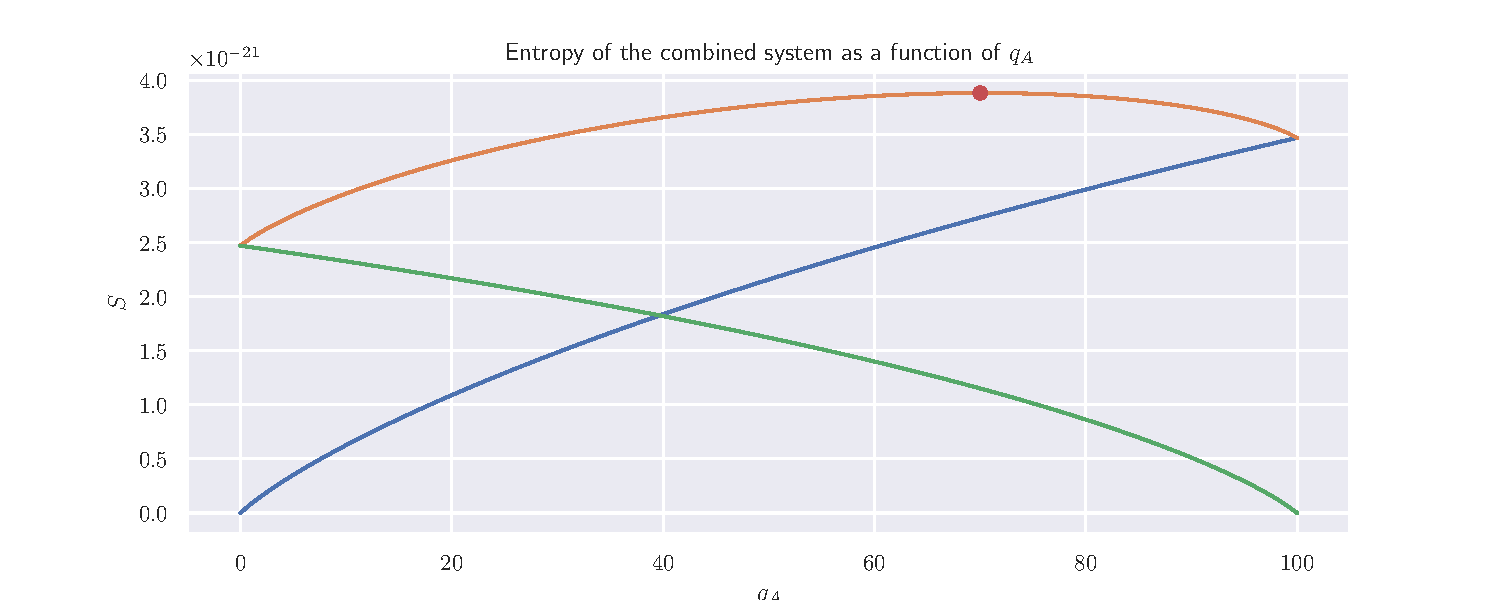
\includegraphics[width=0.5\linewidth]{figures/out.pdf}
		      \caption{\label{fig:Entropies of two systems} Entropies of two systems}
	      \end{figure}

	\item We see that it reached equilibrium when
	      \begin{align}
		      \frac{\partial S_{t}}{\partial q_A} = 0
		      \quad \text{or} \quad \frac{\partial S_{t}}{\partial U_A} = 0
	      \end{align}
	      where the energy $U_A$ is just $q_A$ times a constant.
	\item But $S_t = S_A + S_B$, so
	      \begin{align}
		      \frac{\partial S_A}{\partial U_A} + \frac{\partial S_B}{\partial U_A} = 0 \quad \text{or} \quad
		      \frac{\partial S_A}{\partial U_A} = \frac{\partial S_B}{\partial U_B}
	      \end{align}
	      because $dU_A = -dU_B$
  \item From Figure \ref{fig:Entropies of two systems}, if small values, say $q_A= 10$, for a bit of energy
				passes from solid $B$ to $A$, the entropy gained by $A$ is greater than entropy lost by $B$. Then the overall
				entropy will increase, this happens spontaneously according to the second law.
	\item So energy flows from object with smaller slope into solid with larger slope. We know energy flows from
				object with larger \textit{temperature} into object with a lower one.
	\item So we can define the temperature , with correct units and at constant volume and
				number of particles, as
				\begin{align}
					\frac{1}{T} \equiv \left( \frac{\partial S}{\partial U} \right)_{N,V}
				\end{align}

\end{itemize}




\end{document}
